\section{TikZ}
	 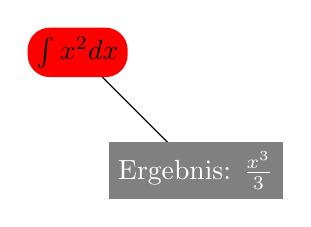
\begin{tikzpicture}
	\draw (0,0)
	node [rounded corners=8pt, fill=red] {$\int x^2 dx$}
	-- (1.5,-1.5)
	node [text=white, fill=gray]
	{Ergebnis: $\frac{x^3}{3}$};
	\end{tikzpicture}
	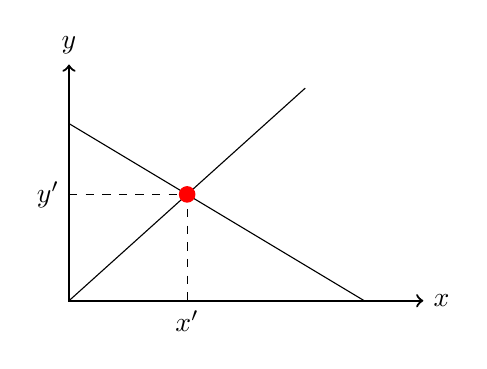
\begin{tikzpicture}[scale=1.5]
	% Draw axes
	\draw [<->,thick] (0,2) node (yaxis) [above] {$y$}
	|- (3,0) node (xaxis) [right] {$x$};
	% Draw two intersecting lines
	\draw (0,0) coordinate (a_1) -- (2,1.8) coordinate (a_2);
	\draw (0,1.5) coordinate (b_1) -- (2.5,0) coordinate (b_2);
	% Calculate the intersection of the lines a_1 -- a_2 and b_1 -- b_2
	% and store the coordinate in c.
	\coordinate (c) at (intersection of a_1--a_2 and b_1--b_2);
	% Draw lines indicating intersection with y and x axis. Here we use
	% the perpendicular coordinate system
	\draw[dashed] (yaxis |- c) node[left] {$y'$}
	-| (xaxis -| c) node[below] {$x'$};
	% Draw a dot to indicate intersection point
	\fill[red] (c) circle (2pt);
	\end{tikzpicture}
	\begin{tikzpicture}
	\datavisualization [school book axes,
	visualize as smooth line,
	y axis={label={$y=x^2$}},
	x axis={label} ]
	
	data [format=function] {
		var x : interval [-1.5:1.5] samples 7;
		func y = \value x*\value x;
	};
	\end{tikzpicture}\\
	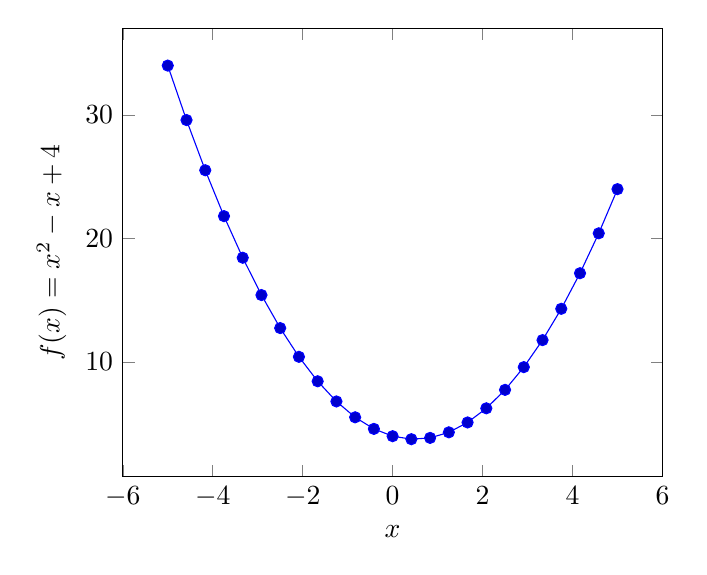
\begin{tikzpicture}
	\begin{axis}[ 
	xlabel=$x$,
	ylabel={$f(x) = x^2 - x +4$}
	] 
	\addplot {x^2 - x +4}; 
	\end{axis}
	\end{tikzpicture}
	\begin{tikzpicture} 
	\begin{axis}[ xlabel=Cost, ylabel=Error] 
	\addplot[color=red,mark=x] coordinates {
		(2,-2.8559703) 
		(3,-3.5301677) 
		(4,-4.3050655) 
		(5,-5.1413136) 
		(6,-6.0322865) 
		(7,-6.9675052) 
		(8,-7.9377747)
	}; 
	\end{axis} 
	\end{tikzpicture}
	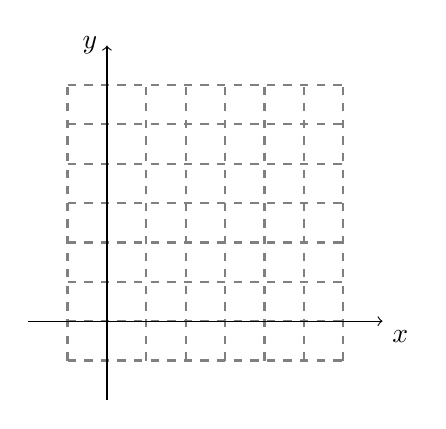
\begin{tikzpicture}[domain=0:2]
	\draw[thick,color=gray,step=.5cm, dashed] (-0.5,-.5) grid (3,3); \draw[->] (-1,0) -- (3.5,0) node[below right] {$x$}; \draw[->] (0,-1) -- (0,3.5) node[left] {$y$};
	\draw plot[id=x] function{x*x};
	\end{tikzpicture}